\section{Decimação, aliasing e folding: o perigo dos 450 kHz}
\label{sec:aliasing}

\subsection{O que a decimação faz com o espectro}

Decimar por um fator $M = 4$ significa manter uma a cada quatro amostras do sinal. Pelo teorema da amostragem, a nova taxa $F_s' = F_s/4 = 480$~kHz só representa sem ambiguidade frequências até a nova frequência de Nyquist:

\begin{equation}
f_{\mathrm{Nyq}}' = \frac{F_s'}{2} = 240 \text{ kHz}.
\end{equation}

No domínio da frequência, a decimação faz o espectro se repetir a cada $F_s' = 480$~kHz. Qualquer componente situada acima de $240$~kHz não desaparece com a operação — ela dobra (\textit{folding}) para dentro da faixa representável, sobrepondo-se ao sinal legítimo. As imagens de uma componente originalmente em uma frequência $f$ aparecem em

\begin{equation}
f_{\mathrm{alias}} = f - k \cdot F_s', \qquad k \in \mathbb{Z},
\label{eq:folding}
\end{equation}

para o valor inteiro de $k$ que traz $f_{\mathrm{alias}}$ para dentro do novo intervalo de Nyquist.

\subsection{A conta do interferente}

Aplicando a Equação~\eqref{eq:folding} ao interferente do cenário, em $450$~kHz, com $k = 1$:

\begin{equation}
f_{\mathrm{alias}} = 450 - 480 = -30 \text{ kHz}.
\end{equation}

Como o espectro é simétrico em módulo, o interferente reaparece em $\pm 30$~kHz — bem no meio do canal útil de $\pm 100$~kHz. O ponto crucial é que o \textit{aliasing} é \textbf{irreversível}: após a decimação, o interferente dobrado em $30$~kHz torna-se matematicamente indistinguível de um componente legítimo do sinal na mesma frequência, e nenhum processamento posterior é capaz de separá-los. Por essa razão, o filtro deve, obrigatoriamente, ser aplicado \emph{antes} do decimador.

A Figura~\ref{fig:diagrama-aliasing} ilustra o mecanismo. Antes da decimação, o interferente ocupa uma posição bem afastada do canal útil. Depois, ele reaparece dentro da faixa protegida, ao lado do sinal que se deseja receber.

\begin{figure}[htb]
\centering
\caption{Dobramento do interferente de $450$~kHz sobre o canal útil ao decimar por $4$.}
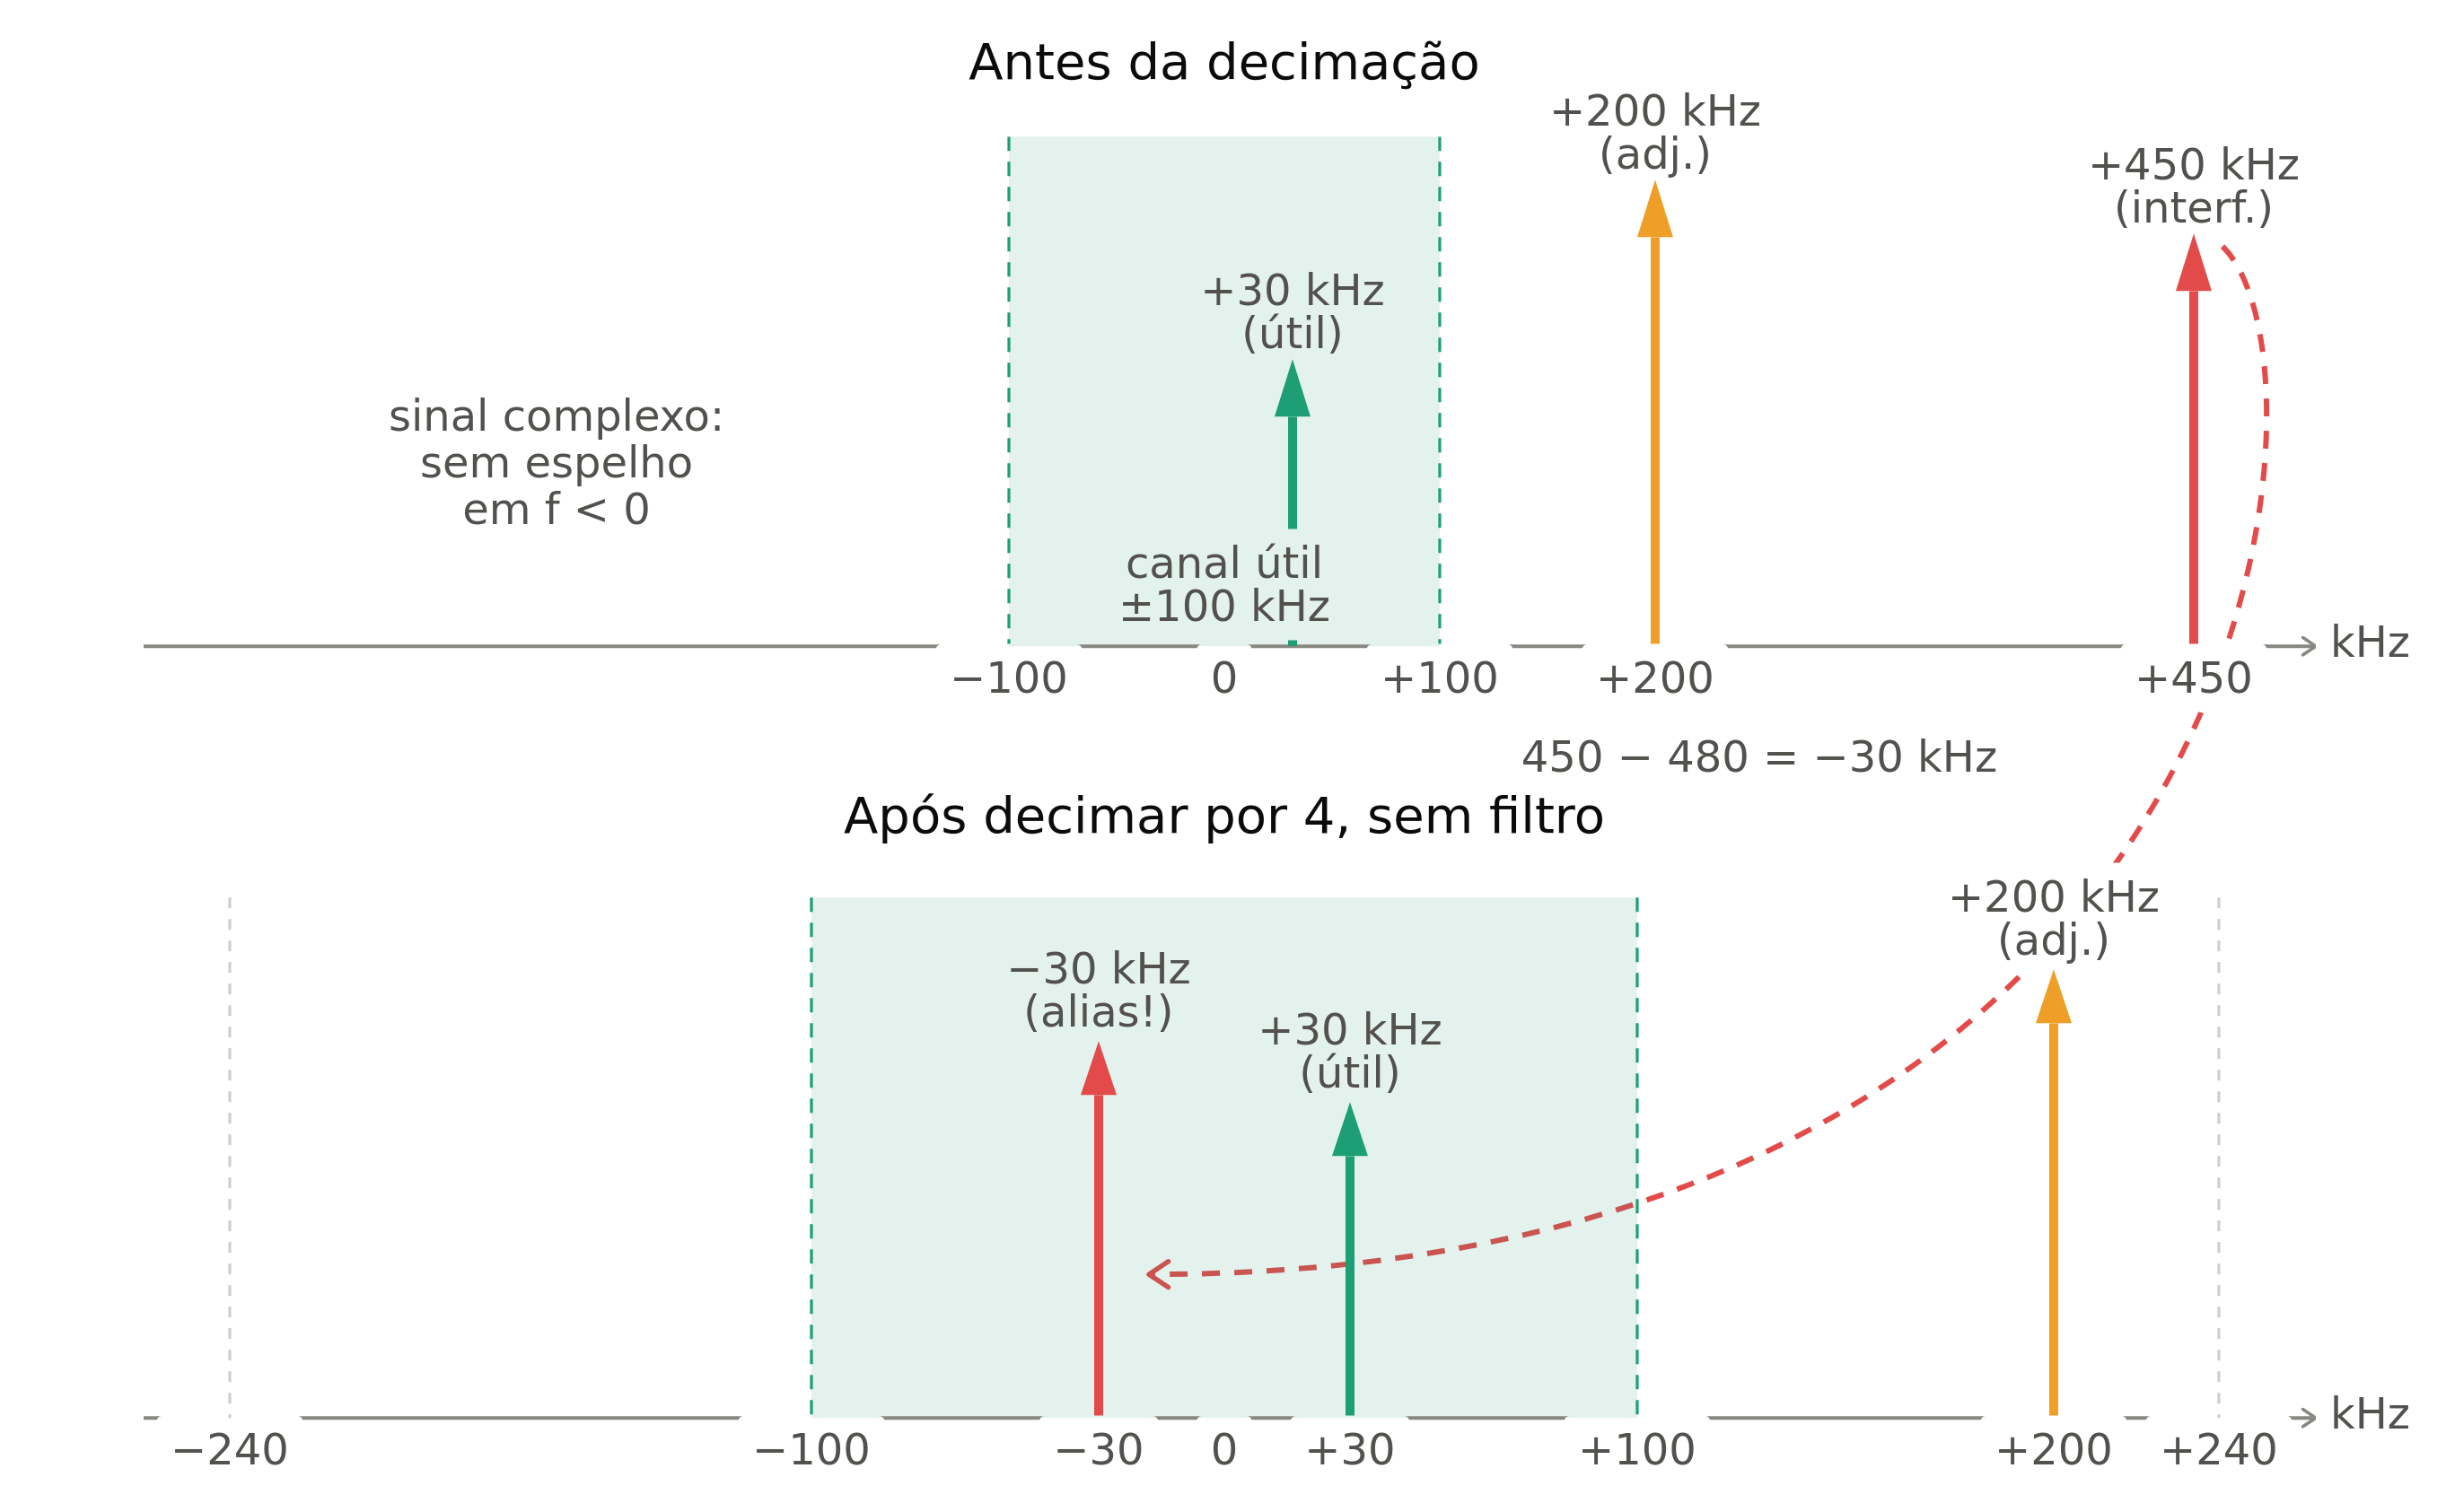
\includegraphics[width=\linewidth]{Imagens/fig00_aliasing_diagrama.png}
\label{fig:diagrama-aliasing}
\fonte{Autoria própria.}
\end{figure}

\subsection{A condição de anti-aliasing e a dupla função do filtro}

Para proteger o canal de $\pm 100$~kHz ao decimar por $4$, o filtro precisa atenuar todas as faixas espectrais que dobram sobre ele:

\begin{equation}
k \cdot 480 \pm 100 \text{ kHz}, \qquad k = 1, 2, \dots
\label{eq:faixas-proibidas}
\end{equation}

isto é, os intervalos de $380$ a $580$~kHz, de $860$ a $960$~kHz, e assim por diante.

Há aqui uma elegância de projeto digna de nota: como a banda de rejeição exigida pela seleção de canal já começa em $200$~kHz --- necessária para bloquear o canal adjacente ---, todas as faixas críticas de \textit{aliasing} dadas pela Equação~\eqref{eq:faixas-proibidas} ficam automaticamente cobertas. O filtro de seleção de canal \emph{é} o filtro de anti-\textit{aliasing}: a decimação não impõe nenhuma exigência adicional sobre a máscara de projeto.

Cabe ainda uma observação: o canal adjacente, centrado em $200$~kHz, situa-se abaixo da nova frequência de Nyquist ($240$~kHz) e, portanto, não sofre \textit{aliasing}. Sua rejeição é exigida por outro motivo — ele constitui interferência co-canal para o classificador de modulação —, e não por risco de dobramento espectral.